\documentclass[a4paper,12pt]{article}

% Include useful packages
\usepackage{fullpage}
\usepackage{graphicx}
\usepackage{amsmath}
\usepackage{amssymb}
\usepackage{amsfonts}
\usepackage{fancyvrb}
\usepackage[sort, numbers]{natbib}
\usepackage{url}

% Helpful commands for mathematical expressions
\newcommand{\dd}[2]{\dfrac{\textrm{d} #1}{\textrm{d} #2}}
\newcommand{\pdd}[2]{\dfrac{\partial#1}{\partial#2}}
\newcommand{\pddb}[2]{\left( \dfrac{\partial#1}{\partial#2} \right)}
\newcommand{\boldnabla}{\mbox{\boldmath$\nabla$}}
\renewcommand{\vec}[1]{\mathbf{#1}}
\newcommand{\uvec}[1]{\mathbf{#1}}
\renewcommand{\and}{ \text{and} }
\newcommand{\for}{ \text{for} }

% Helpful commands for authors' notes
\newcommand{\completed}{[Completed]}
\newcommand{\todo}{[Started]}
\newcommand{\tostart}{[Still to do]}
\newcommand{\authornote}[2]{{\bf [#1: #2]}}
\newcommand{\alex}[1]{\authornote{Alex}{#1}}
\newcommand{\ozzy}[1]{\authornote{Ozzy}{#1}}

\begin{document}

% Make title
\title{The influence of cell level model choice on the outcome of multiscale simulations}
\author{J.M. Osborne$^{1,2,\dagger}$\footnote{Corresponding author ({\tt James.Osborne@comlab.ox.ac.uk})} ,
A.G. Fletcher$^{2,3,\dagger}$,  
P.K. Maini$^{2,3}$ and D.J. Gavaghan$^{1,2}$ + TBC}
\date{{\small 
\textit{$^{1}$Oxford University Computing Laboratory, Parks Road, Oxford OX1 3QD, UK}\\
\textit{$^{2}$Oxford University Department of Biochemistry, South Parks Road, Oxford OX1 3QU, UK}\\
\textit{$^{3}$Oxford University Mathematical Institute, 24-29 St Giles', Oxford OX1 3LB, UK}\\
\textit{$^{\dagger}$Joint first authors.}}}
\maketitle


\begin{abstract}
\ozzy{The key results intended for this paper are:
\begin{itemize}
\item{A comparison of different cell-level modelling approaches (cellular Potts model, 
centre dynamics models and vertex dynamics models)}
\item{Brief discussion of the implementation of these approaches within the Chaste framework}
\item{Comparison of the different Chaste codes used to create example simulations}
\end{itemize}

Possible journal is SIAM: Multiscale Modeling and Simulation 
}

\end{abstract}
\clearpage

%%%%%%%%%%%%%%%%%%%%%%%%%%%%%%%%%%%%%%%%%%%%%%%%%%
%%%%%%%%%%%%%%%%%%%% Section %%%%%%%%%%%%%%%%%%%%%
%%%%%%%%%%%%%%%%%%%%%%%%%%%%%%%%%%%%%%%%%%%%%%%%%%

\tableofcontents
\clearpage

%%%%%%%%%%%%%%%%%%%%%%%%%%%%%%%%%%%%%%%%%%%%%%%%%%
%%%%%%%%%%%%%%%%%%%% Section %%%%%%%%%%%%%%%%%%%%%
%%%%%%%%%%%%%%%%%%%%%%%%%%%%%%%%%%%%%%%%%%%%%%%%%%
\section{Introduction \tostart} \label{sec1}

\begin{itemize}
\item Short review of cell-based models 
\item Where models come from 
\item simulation methods
\item Why we need a consistent simulation framework
\end{itemize}

\alex{What other comparison papers (if any) have been written?}

The remainder of this paper is structured as follows...

%%%%%%%%%%%%%%%%%%%%%%%%%%%%%%%%%%%%%%%%%%%%%%%%%%
%%%%%%%%%%%%%%%%%%%% Section %%%%%%%%%%%%%%%%%%%%%
%%%%%%%%%%%%%%%%%%%%%%%%%%%%%%%%%%%%%%%%%%%%%%%%%%
\section{Cell based models of biological tissues \tostart} \label{sec:cell_level_models}

\begin{itemize}
  \item CA
  \item Potts
  \item Cell centre
  \item Cell vertex
\end{itemize}

%%%%%%%%%%%%%%%%%%%%%%%%%%%%%%%%%%%%%%%%%%%%%%%%%%
%%%%%%%%%%%%%%%%%%%% Section %%%%%%%%%%%%%%%%%%%%%
%%%%%%%%%%%%%%%%%%%%%%%%%%%%%%%%%%%%%%%%%%%%%%%%%%
\section{Framework structure \todo} \label{sec:computational_framework}

The multiscale modelling framework consists of three main interacting scales: the cellular scale; 
the subcellular scale; and the tissue scale.

\begin{description}
\item [The cellular (meso) scale.] {The cell is the central element of the framework.} 

    \begin{description}
	    \item [Cellular Automata.]{ The simplest form of cellular modelling,
    cells are represented as points on a lattice and rules constructed in order for
    each cell to divide, move or die. Cells can only divide in to neighbouring spaces
    on the lattice. Some of the issues with this type of modelling include: effects felt at distance; 
    fixed regular lattice
    geometry; growth is lattice dependent -- 4 point $\rightarrow$ star and 8 point
    $\rightarrow$ octagon; and finally you can't consider stress in the tissue.}

	    \item [Cellular Potts.]{An extension of cellular automata model is the
    Cellular Potts Model, in which cells are composed of a number of lattice points, and
    the cell shape is evolved by minimizing the energy which is calculated by
    imposing constraints due to chemotaxis etc. This form of modelling is utilised
    in the CompuCell3D modelling package produced at Indiana University.}

	    \item [Overlapping sphere models.]
	    {See the work of Drasdo \emph{et al}, for example \citep{Drasdo2007Role}.
    Cells are modelled as overlapping spheres and energy minimization is used to
    evolve the system, cells can divide depending on binary rules or buy using a
    cell cycle model. The software package MASON from UCSF deals with this type of modelling. 
    Extensions include ellipses with varying radii and orientation. 
    Chaste functionality for this is discussed in a recent computational study by 
    \citet{Pathmanathan2009Computational} of the mechanical properties of this class of model.}

	    \item [Subcellular Element Method.]{This is an extension of the
    overlapping spheres approach and treats cells as being composed of subcellular
    elements with different interactions between inter-cell and intra-cell elements 
    \citep{Newman2005Modeling,Sandersius2008Modeling} }

	    \item[Centre Dynamics Tessellation Models.] This was the first class of cell-based model 
	    added to Chaste \citep{Leeuwen2009Integrative} and are based on the model 
	    presented by \citet{Meineke2001Cell}.

	    \item[Vertex Dynamics Models.] Cells defined by polygons
    and movement determined by energy minimization. Currently implemented in Chaste in two 
    dimensions \citep{Osborne2010Hybrid}.

	    \item[Finite Element Models.] Generalization of vertex where cell
    represented as collections of moving and deforming elements -- tetrahedra for
    example.	

    \end{description}

    \item [The subcellular (micro) scale.] {The behaviour of cells is dictated by modelling 
    the numerous subcellular processes occurring within the cell. The main modelling paradigm 
    is to use reaction networks rendered into ODEs which interacting with cell level through 
    the cell cycle and also directly through properties such as cell size, shape and motility 
    etc. Other methods include: stochastic ODEs; PDEs; or fully stochastic networks which 
    representing the transport and use of substrates within cells.}

    \item [The tissue (macro) scale.] {Modelling of inter-cellular signalling, or nutrient 
    transfer can be considered by using reaction diffusion equations, 
    which are solved on the growing domain (defined by the cells) with cells acting as sinks 
    and sources \ozzy{We don't have PDEs for vertex yet: we should 
    reference Aaron's paper here \citep{SmithSubmitted}}.}
\end{description}

The advantage of such a framework is that once you have implemented a particular subcellular 
model you can use it in all possible cell level models.

%%%%%%%%%%%%%%%%%%% SubSection %%%%%%%%%%%%%%%%%%%
\subsection{Computational structure \todo} \label{sec:computational_structure}
Chaste (Cancer, Heart and Soft Tissue Environment) is a collaborative software
development project, which is designed to act as a high-quality multi-purpose library
supporting computational simulations for a wide range of biological problems \citep{Pitt-Francis2008Chaste}. 
In this context, ‘high-quality’ means that the software is extensible, robust, fast, accurate and
maintainable and uses state-of-the-art numerical techniques. It is also open-source, so
can be adapted by other developers. Chaste has been developed by a multidisciplinary
team including mathematicians and software engineers. This ensures that the code is
well-structured as a piece of software, while at the same time practical and useful as a
computational modelling tool. While it is a generic extensible library, to date attention
has focused on the fields of cardiac electrophysiology and tumor growth \citep{Pitt-Francis2009Chaste}. 
Further details on Chaste are available at \url{http://web.comlab.ox.ac.uk/chaste}.


\begin{figure}[tbhp]
        \centering
        \setlength{\unitlength}{1cm}
        \begin{picture}(10,10)
              \put(0,0){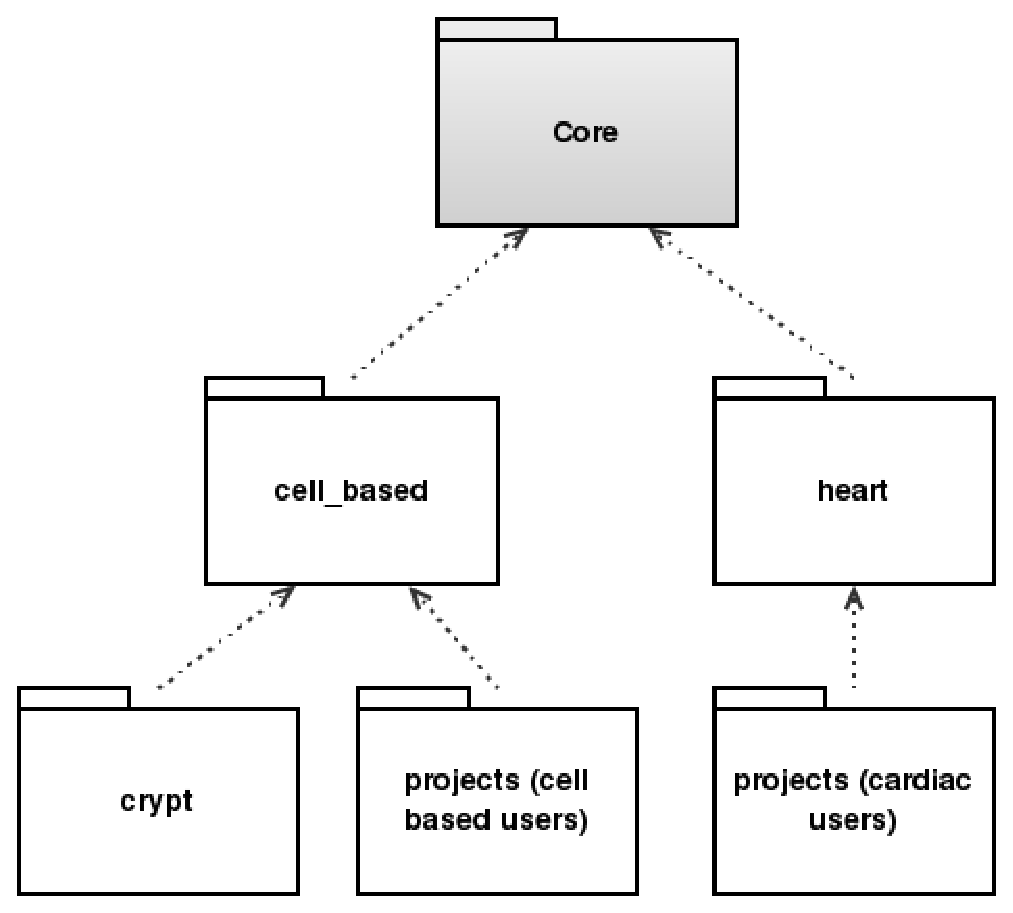
\includegraphics[width=10cm]{Figs/ChasteStructure}}
	      \put(1.5,5.0){\huge{Need to change this and}}
              \put(0.0,3.5){\huge{add Crypt and projects folders.}}
        \end{picture}
        \caption{Schematic diagram of Chaste code base.} 
       \label{fig:ChasteStructure}
\end{figure}

%%%%%%%%%%%%%%%%%%% SubSection %%%%%%%%%%%%%%%%%%%
\subsection{Structure of code \todo} \label{sec:code}
To set up a cell-based simulation within Chaste you need to instantiate a collection of objects which specify the properties of the simulation. 
The following seven objects can be defined for a simulation to be undertaken:
\begin{description}
  \item [Mesh,] the structural information for the simulation, the initial epithelial layer 
  layout is defined here.
  \item [Cells,] a collection of cells to be associated with the mesh. Contain all the subcellular 
  machinery. The initial conditions for  subcellular models are defined here.
  \item [Cell population,] associated the cells with the mesh and provides a mechanism for 
  cells to know their location.
  \item [Simulation,] takes in the cell population and implements the rules for evolution of 
  the system.
  \item [Forces,] these are passed in to the simulation and dictate the way the vertices move. 
  This is the mechanism for selection of the type of vertex dynamics model. Multiple forces 
  can be applied allowing the introduction of processes like chemotaxis.
  \item [*Cell killers,] these are passed to the simulation and define how cells die. Multiple 
  killers can be used at the same time for example to represent random death and death due to 
  sloughing.
  \item [*Boundary Conditions (BCS),] these are passed to the simulation and define any fixed 
  restrictions on how the cells can move. Multiple conditions can be used at the same time.
\end{description}
The stared objects are optional as you may not want to have cells being removed from the simulation and the growth may be unconstrained. 


\begin{figure}[tbhp]
        \centering
        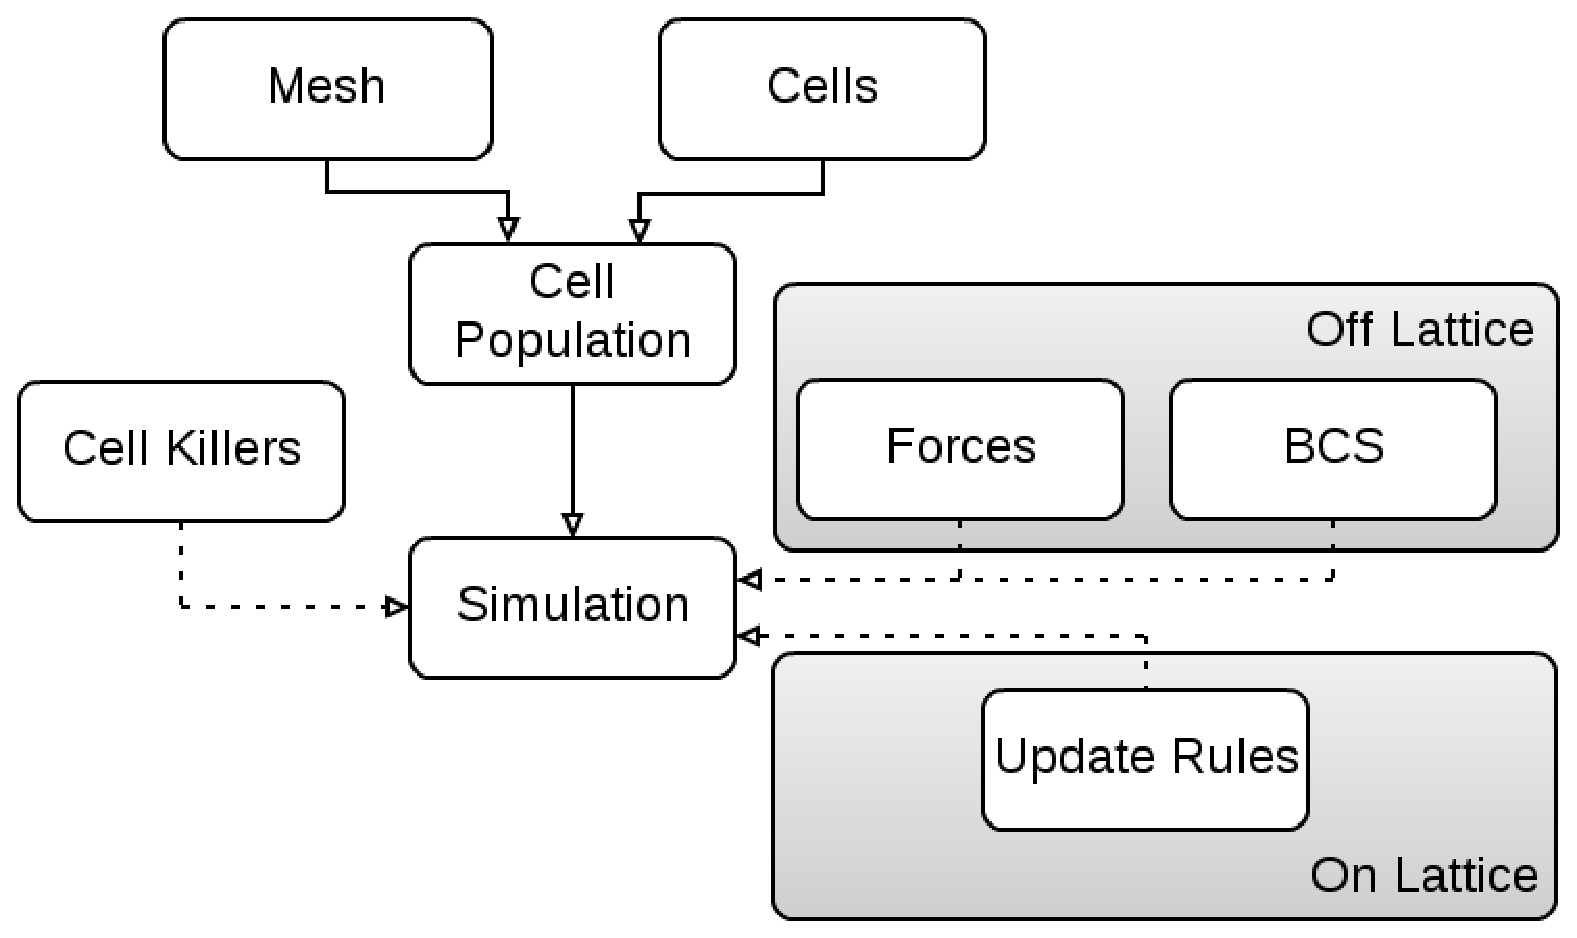
\includegraphics[width=10cm]{Figs/CellBasedStructure}
        \caption{Schematic diagram of the framework showing the separate components of the simulations and the communication between the classes.} 
       \label{fig:SimulationComponents}
\end{figure}


%%%%%%%%%%%%%%%%%%%%%%%%%%%%%%%%%%%%%%%%%%%%%%%%%%
%%%%%%%%%%%%%%%%%%%% Section %%%%%%%%%%%%%%%%%%%%%
%%%%%%%%%%%%%%%%%%%%%%%%%%%%%%%%%%%%%%%%%%%%%%%%%%
\section{Example simulations \todo} \label{sec:example_simulations}
\begin{itemize}
  \item Monolayer
  \item Spheroid 
  \item crypt??
\end{itemize}

%%%%%%%%%%%%%%%%%%% SubSection %%%%%%%%%%%%%%%%%%%
\subsection{Demonstration of growing monolayer \todo} \label{sec:growing_domain}
\begin{itemize}
  \item Demonstrate basic functionality
  \item Example of growing monolayer with void removal, sloughing? etc. 
  \item Show differneces in code from model to model
\end{itemize}
\begin{small}
\begin{Verbatim}[frame=single, numbers=left, numbersep=2pt]
void TestVertexMonolayerWithRandomBirthAndDeath() throw (Exception)
{
    // Create a simple 2D vertex mesh
    HoneycombVertexMeshGenerator generator(5, 5);
    MutableVertexMesh<2,2>* p_mesh = generator.GetMesh();

    // Set up cells, one for each element in the vertex mesh
    std:vector<CellPtr> cells;
    CellsGenerator<StochasticDurationGenerationBasedCellCycleModel, 2>
        cells_generator;
    cells_generator.GenerateBasic(cells,p_mesh->GetNumElements());

    // Create cell population
    VertexBasedCellPopulation<2> cell_population(*p_mesh, cells);

    // Set up cell-based simulation
    CellBasedSimulation<2> simulator(cell_population);
    simulator.SetOutputDirectory("TestVertexMonolayer");
    simulator.SetEndTime(40);

    // Create a force law and pass it to the simulation
    NagaiHondaForce<2> force_law;
    simulator.AddForce(&force_law);

    // Create cell killer and pass it to the simulation
    RandomCellKiller<2> random_cell_killer(&cell_population, 0.01);
    simulator.AddCellKiller(&random_cell_killer);

    // Run simulation
    simulator.Solve();
}
\end{Verbatim}
\end{small}

%%%%%%%%%%%%%%%%%%% SubSection %%%%%%%%%%%%%%%%%%%
\subsection{Demonstration of cell sorting \tostart} \label{sec:cell_sorting}
\begin{itemize}
 \item Potts and Vertex comparison.
\end{itemize}

%%%%%%%%%%%%%%%%%%% SubSection %%%%%%%%%%%%%%%%%%%
\subsection{Demonstration of spheroid \tostart} \label{sec:spheroid}
\begin{itemize}
 \item Include nutrient diffusion.
\end{itemize}

%%%%%%%%%%%%%%%%%%% SubSection %%%%%%%%%%%%%%%%%%%
\subsection{Demonstration of crypt \tostart} \label{sec:crypt}
\begin{itemize}
  \item 2D cylindrical crypt in each modality. 
  \item 3D node based crypt.
\end{itemize}


%%%%%%%%%%%%%%%%%%%%%%%%%%%%%%%%%%%%%%%%%%%%%%%%%%
%%%%%%%%%%%%%%%%%%%% Section %%%%%%%%%%%%%%%%%%%%%
%%%%%%%%%%%%%%%%%%%%%%%%%%%%%%%%%%%%%%%%%%%%%%%%%%
\section{Discussion \tostart} \label{sec:discussion}

%%%%%%%%%%%%%%%%%%%%%%%%%%%%%%%%%%%%%%%%%%%%%%%%%%
%%%%%%%%%%%%%%%%%%%% Section %%%%%%%%%%%%%%%%%%%%%
%%%%%%%%%%%%%%%%%%%%%%%%%%%%%%%%%%%%%%%%%%%%%%%%%%
\section*{Acknowledgements \todo}
JMO and AGF are funded through the OCISB project (BB/D020190/1). JMO is also supported by the Life Sciences Interface and Systems Biology Doctoral Training Centres (EP/E501605/1 and EP/G50029/1 respectively).

\clearpage

%%%%%%%%%%%%%%%%%%%%%%%%%%%%%%%%%%%%%%%%%%%%%%%%%%
%%%%%%%%%%%%%%%%%%%% Section %%%%%%%%%%%%%%%%%%%%%
%%%%%%%%%%%%%%%%%%%%%%%%%%%%%%%%%%%%%%%%%%%%%%%%%%
\bibliography{comparison_refs}{}
\bibliographystyle{apalike}

\end{document}
